\documentclass[handout]{beamer}
 
\usepackage[utf8]{inputenc}
\usepackage{mathtools}
\usepackage{tikz}

\usetheme{CambridgeUS}
% \useoutertheme{split}
\setbeamertemplate{title page}[default][colsep=-4bp,rounded=true]

% only inlcude the current secition in the header
\AtBeginSection{
    \begin{frame}
        \tableofcontents[sections=\value{section}, sectionstyle=show/show]
    \end{frame}
}

\usetikzlibrary{calc,shapes}
\usetikzlibrary{fit,positioning,decorations.pathreplacing,calligraphy}

\tikzstyle{key}=[circle, thin, minimum width=\ln, minimum height=\hn, draw=black, fill=white, inner sep=0cm, anchor=north]
\tikzstyle{fts}=[key,fill=gray!50,minimum width=0.8*\ln]
\tikzstyle{hash}=[key,rectangle, anchor=north]

\renewcommand{\ln}{6mm} % largeur de noeud
\newcommand{\hn}{6mm}    % hauteur de noeud
\renewcommand{\le}{5mm} % largeur de l'espace
\newcommand{\he}{8mm}   % hauteur de l'espace

\newcommand{\hasharrow}[2]{ \draw (H#2.north) -- ($(H#2.north)+(0,.5*\he)$) -- ($(H#1.south)+(0,-.5*\he)$) -> (H#1.south); }
\newcommand{\keyhasharrow}[2]{ \draw (K#2.north) -- ($(K#2.north)+(0,.5*\he)$) -- ($(H#1.south)+(0,-.5*\he)$) -> (H#1.south); }
\newcommand{\signarrow}[2]{ \draw (K#1.south) edge[dashed,->] (H#2.north); }


%Information to be included in the title page:
\title{Block Chain}
\author{Rohit Musti}
\institute{CUNY - Hunter College}
\date{\today}
 
\begin{document}
 
\frame{\titlepage}

% Outline frame
\begin{frame}{Table of Contents}
  \tableofcontents
\end{frame}

\section{Disclaimer}

\begin{frame}{Disclaimer}
    \begin{itemize}
        \item \pause These slides do not reflect my personal opinion on the viability or effectiveness of blockchain technology or cryptocurrencies
        \item \pause Please carefully review any investments into cryptocurrencies and make sure you have an extremely clear understanding of why you believe that investment will yield a significant enough return to justify the risk of it failing
        \item \pause There are many fraudulent scams out there trying to take your money through cryptocurrency schemes and a few honest actors trying to do what they believe is right. At times it can be hard to distinguish them
        \item \pause I am also (at the time of this slide creation) not personally invested in any blockchain technologies so I don't have any financial incentive to see these new ways of transacting succeed. If that changes, this slide will be updated.
    \end{itemize}
\end{frame}

\section{Overview}

\begin{frame}{Blockchain}
    \begin{itemize}
        \item \pause \textit{definition}: a persistent, transparent, public, append-only ledger that is managed using a mechanism that allows distributed group of actors to work together to verify the ledger and new additions without trusting one another and such that no one actor can dominate who controls the ledger
        \item \pause \textit{use}: to allow a group of actors that do not inherently trust one another to have a mechanism for confirming that transactions did in fact happen
        \item \pause this isn't inherently limited to just transactions, theoretically any digital exchange of information can be put on a distributed ledger like this
    \end{itemize}
\end{frame}

\begin{frame}{Why?}
    \begin{itemize}
        \item \pause Let's pretend we cannot trust institutions
        \item \pause For example, what if you learned in a cryptography class taught by a very cool professor that the US government has, throughout its history, actively tried to undermine the cyber security of its citizens (cough cough NSA)
        \item \pause What if, Wells Fargo was found guilty of employees opening up fake accounts in customers names, signing them up for credit cards, forging their signatures, and secretly transferring the customers money without their permission between 2002 - 2016. What if this very same bank was found guilty of charging mortgage customers unnecessary fees and forced auto-loan borrowers to buy unnecessary insurance.
    \end{itemize}
\end{frame}

\begin{frame}{Why?}
    \begin{itemize}
        \item \pause If we cannot trust institutions to safely handle our transactions, we need to hold them accountable through the mechanisms we have agreed up on socially (courts, laws, regulators, etc.).
        \item \pause If those mechanisms fail, we either need to revise those systems or overthrow those in power
        \item \pause Systemic change is hard in most western countries and revolutions tend to be bloody and violent, so having our own mechanism for transferring and maintaining money would be incredibly valuable. This is the central argument for crypto-currencies.
    \end{itemize}
\end{frame}

\section{Mechanisms}

\begin{frame}{Distributed Ledger: Example}
    \begin{itemize}
        \item \pause If you exchange money with your friends, exchanging cash or venmo/zelle-ing all of the time is inconvenient. So you might keep a ledger to keep track of who owes who what money (kind of like a bar tab).
        \item \pause Every so often, you calculate how much money you spent vs received. If you spent more than you received, you put money in the pot. If you received more than you spent, you take money from the pot.
    \end{itemize}
\end{frame}

\begin{frame}{Distributed Ledger: Weak Protocol}
    \begin{enumerate}
        \item \pause Anyone can add lines to the ledger.
        \item \pause At the end of a time period (every two weeks, money is exchanged based on the ledger record)
    \end{enumerate}
\end{frame}

\begin{frame}{Distributed Ledger: Weak Protocol Weaknesses + Solutions}
    \begin{enumerate}
        \item \pause Anyone can add lines to the ledger, therefore Bob could write \textit{Alice owes bob \$100} without Alice having sent Bob \$100
        \item \pause Solution: Unique Ids + Digital Signatures. If messages have unique ids you cannot replicate them without changing the ids and if Alice signs all transactions with a digital signature, then we can guarantee that the transaction came from the person controlling her secret key.
        \item \pause Is this actually the same as Alice sending it? No. What if she leaves her secret key at a coffee shop or someone guesses it?
    \end{enumerate}
\end{frame}

\begin{frame}{Distributed Ledger: Weak Protocol Weaknesses + Solutions}
    \begin{enumerate}
        \item \pause Anyone can add lines to the ledger
        \item \pause At the end of a time period (every two weeks, money is exchanged based on the ledger record)
        \item \pause Only signed, unique ID transactions are considered valid
    \end{enumerate}
\end{frame}

\begin{frame}{Distributed Ledger: Weak Protocol Weaknesses + Solutions}
    \begin{enumerate}
        \item \pause What if someone refuses to settle up cash?
        \item \pause What if they send hundreds of dollars at a time to people and then refuse to actually pay up when the time period ends.
        \item \pause Introduce a mechanism to stop someone from spending money that they do not have. (maybe at the begining of the time period everyone has to add money to their account that serves as their account total and this is recorded on the ledger too)
    \end{enumerate}
\end{frame}

\begin{frame}{Distributed Ledger: Weak Protocol Weaknesses + Solutions}
    \begin{enumerate}
        \item \pause Anyone can add lines to the ledger
        \item \pause At the end of a time period (every two weeks, money is exchanged based on the ledger record)
        \item \pause Only signed, unique ID transactions are considered valid
        \item \pause No overspending.
    \end{enumerate}
\end{frame}

\begin{frame}{Distributed Ledger: Weak Protocol Weaknesses + Solutions}
    \begin{itemize}
        \item \pause Who controls the ledger document?
        \item \pause you distribute it, everyone gets their own copy of the ledger
        \item \pause Once a transaction happens, it is broadcasted and everyone else records that transaction
        \item \pause In order to verify that a transaction actually happened, you would want to know that everyone else received the very same transaction.
        \item \pause How can we guarantee that everyone else is receiving the same transactions and recording them correctly? This is the problem solved in the original Bitcoin white paper
    \end{itemize}
\end{frame}

\begin{frame}{Distributed Ledger: Trust}
    \begin{enumerate}
        \item \pause How can we guarantee everyone is recording the same transactions?
        \item \pause You trust the ledger that has had the most computational work put into it 
        \item \pause Specifically, we append a number to the end of a block of transactions such that if you take the SHA-256 hash function of those messages with that number appended at the end, you get a resulting hash where the first 30 digits are zeros (number of zeros increased to keep total time to compute a block to around 10 minutes). 
        \item \pause This allows us to guarantee that whoever computed the hash function put in an enormous amount of work because they had to essentially brute force until they got that number. This is "proof of work".
    \end{enumerate}
\end{frame}

\begin{frame}{Distributed Ledger: Trust}
    \begin{enumerate}
        \item \pause Organize ledger into a series of blocks
        \item \pause Each block needs to have this proof of work number tacked on the end to be valid
    \end{enumerate}
\end{frame}

\begin{frame}{Distributed Ledger: Ordering}
    \begin{enumerate}
        \item \pause Blocks need to be in order though! What if these blocks are verified with proof of work but don't have any ordering. No way to determine if overspending
        \item \pause Therefore, each block has to contain the previous block's hash output in its header
        \item \pause this results in the "block chain"
    \end{enumerate}
\end{frame}

\begin{frame}{Distributed Ledger: Mining}
    \begin{itemize}
        \item \pause In order to incentivize block creators to compute these hashes, we have to allow them to prepend a transaction to the top of every transaction giving them some kind of currency total
        \item \pause What miners do is they listen for transactions, create blocks, broadcast blocks, and get rewarded for this little lottery.
        \item \pause If you want to make transactions, what you do is you listen for miners broadcasting blocks and add it onto your chain. If there are two conflicting blocks, then you take whicheveryone is part of the longest pre-existing chain, ties are broken by whichever one is made longer next
        \item \pause Despite there being no centralized authority, whichever blockchain has the most work into it, is the longest, 
        \item \pause Also, the reward for computing a block decreases by half every 210 thousand transactions so there will never be more than 21 million bitcoin in existence
    \end{itemize}
\end{frame}

\begin{frame}{Longest Chain Security}
    \begin{itemize}
        \item \pause Let's say you alter a transaction in a block you receive as a miner to trick one person into thinking you sent them money and make everyone else not know (i.e. you send them a fraudulent block) 
        \item \pause You would have to keep sending that person new blocks based on your fraudulent block. At some point you will fall behind the rest of the miners and will not be able to keep beating them
        \item \pause Unless you have around half the computer power of the entire chain, then you will quickly fall behind everyone else
        \item \pause In general, you shouldn't trust a new block immediately, you want to trust it every it has a sufficient number of blocks after it
    \end{itemize}
\end{frame}

\begin{frame}{Flaws}
    \begin{itemize}
        \item \pause Bitcoin blocks are restricted to 2,400 transactions and a new block is computed roughly every ten minutes, by comparison VISA can handle 24 thousand a second
        \item \pause Miners also prefer transactions that give them a transaction fee/tip ontop of their regular reward, this means that the transaction fee to get into that 2,400 transaction block is going to go up over time
        \item \pause blockchain is growing in size infinitely
    \end{itemize}
\end{frame}

\section{Merkle Trees}

\begin{frame}{Merkle Tree}
    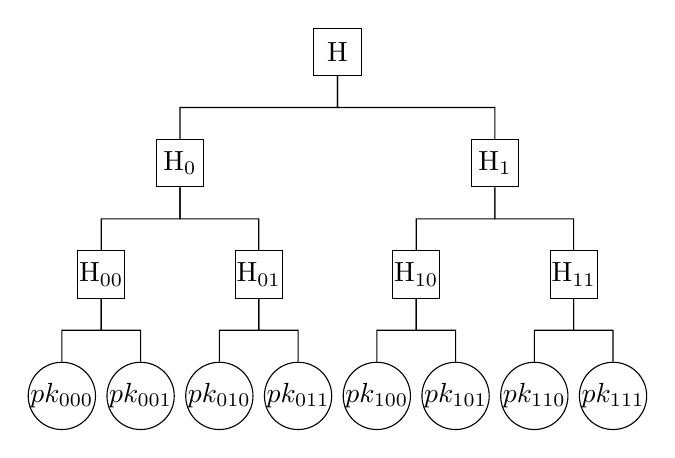
\begin{tikzpicture}
        \node[hash] (H) at (0,0) {H};
        \foreach \i in {0,1}%
        {%
            \node[hash] (H\i) at ($(H.south)+(8*\i*\le-4*\le,-\he)$) {H${}_\i$};%
            \hasharrow{}{\i};
            \foreach \k in {0,1}{
                \node[hash] (H\i\k) at ($(H\i.south)+(4*\k*\le-2*\le,-\he)$) {H${}_{\i\k}$};
                \hasharrow{\i}{\i\k};
                 \foreach \l in {0,1}{
                      \node[key] (H\i\k\l) at ($(H\i\k.south)+(2*\l*\le-1*\le,-\he)$) {$pk_{\i\k\l}$};
                    \hasharrow{\i\k}{\i\k\l};
                }
            }
        }
       
       \end{tikzpicture}
\end{frame}

\begin{frame}{Merkle Tree}
    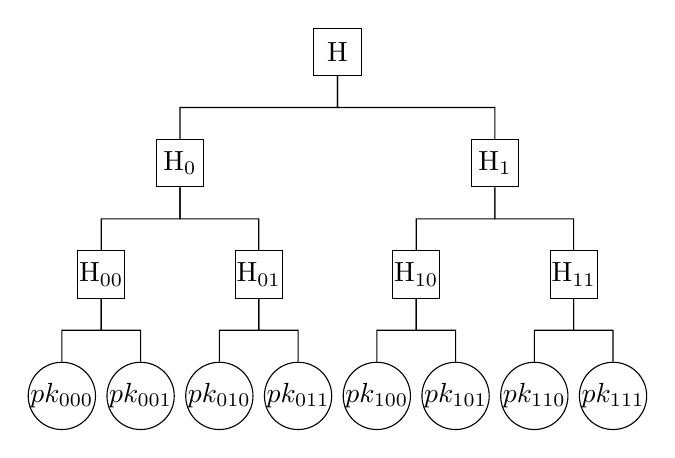
\begin{tikzpicture}
        \node[hash] (H) at (0,0) {H};
        \foreach \i in {0,1}%
        {%
            \node[hash] (H\i) at ($(H.south)+(8*\i*\le-4*\le,-\he)$) {H${}_\i$};%
            \hasharrow{}{\i};
            \foreach \k in {0,1}{
                \node[hash] (H\i\k) at ($(H\i.south)+(4*\k*\le-2*\le,-\he)$) {H${}_{\i\k}$};
                \hasharrow{\i}{\i\k};
                 \foreach \l in {0,1}{
                      \node[key] (H\i\k\l) at ($(H\i\k.south)+(2*\l*\le-1*\le,-\he)$) {$pk_{\i\k\l}$};
                    \hasharrow{\i\k}{\i\k\l};
                    \pause
                }
            }
        }
       \end{tikzpicture}
\end{frame}

\end{document}